% CPU-generated numerical companion. Compile twice for cross-references.
\documentclass[11pt]{article}
\usepackage[paperwidth=29.7cm,paperheight=28cm,margin=1.6cm]{geometry}
\usepackage{booktabs,array,graphicx,amsmath,amsfonts,tikz,natbib}
\usetikzlibrary{arrows.meta,positioning,shapes.geometric}
\usepackage[T1]{fontenc}
\setlength{\parindent}{0pt}
\begin{document}
\begin{figure*}[t]
\centering
\input{figures/d4-development}
\caption{\textbf{Development of the 20M full-sequence baseline (one training seed).} The line ends at the split used for larger block models (one quarter AR). The 37M variant (open circle) uses the same split and token budget as the 20M model. Both receive about 461M tokens because the budget excludes the extra value embeddings.}
\label{fig:d4-development}
\end{figure*}

\clearpage
\begin{table*}[t]
\input{tables/component-budget-rows}
\centering\small
\setlength{\tabcolsep}{4pt}
\renewcommand{\arraystretch}{1.12}
\begin{tabular}{@{}lllrrl@{}}
\toprule
Component & Matched control & Budget & $\Delta$ BPB & 95\% interval & Interpretation \\
\midrule
\exhibitrows
\bottomrule
\end{tabular}
\caption{\textbf{Which published components improve next-token prediction at 20M parameters?} Negative differences favor the component. All pairs score the same 32 documents with masks to the block boundary. Intervals resample documents jointly across the two fitted seeds. TPP includes the AR parent when used. The two fixed-block controls differ in both trainer and attention within each clean 32-token block. The equal-token rows reuse the same Fast-v2 checkpoints. The final Fast-v2 row retains the block-causal control and matches estimated conversion FLOPs within 1\%.}
\label{tab:component-budget}
\end{table*}

\clearpage
\begin{figure*}[!t]
\centering
\resizebox{\textwidth}{!}{\begin{tikzpicture}[font=\small, next/.style={blue!75!black}, recon/.style={teal!75!black}]
\input{figures/transfer-marks}
\def\axes{
  \foreach \tick/\labeltext in {-.08/-.08,-.04/-.04,0/0,.02/+.02}{
    \draw[black!13] (\tick,-.20)--(\tick,2.80);
    \node[below,font=\footnotesize] at (\tick,-.20) {$\labeltext$};}
  \draw[black!55] (0,-.20)--(0,2.80);}
\def\rowname#1#2{\node[anchor=east,font=\footnotesize] at (-.083,{2.60-.48*#1}) {#2};}
\def\fullmark#1#2{
  \draw[black!35] (#2,{2.60-.48*#1})--(0,{2.60-.48*#1});
  \node[diamond,fill=black!70,inner sep=1.65pt] at (#2,{2.60-.48*#1}) {};}
\def\nexttokenmean#1#2{\fill[next] (#2,{2.69-.48*#1}) circle[radius=2pt];}
\def\reconstructmean#1#2{\node[rectangle,draw=teal!75!black,fill=white,inner sep=1.65pt] at (#2,{2.51-.48*#1}) {};}
\def\nexttoken#1#2#3#4{\draw[next,line width=.8pt] (#3,{2.69-.48*#1})--(#4,{2.69-.48*#1});\nexttokenmean{#1}{#2}}
\def\reconstruct#1#2#3#4{\draw[recon,line width=.8pt] (#3,{2.51-.48*#1})--(#4,{2.51-.48*#1});\reconstructmean{#1}{#2}}
\foreach \xx/\yy/\titletext/\subtitle/\marks in {
  0/4.70/A. Full-sequence diffusion/50\% of training tokens allocated to AR/Full,
  8.0/4.70/B. Block diffusion by size/25\% AR · 32 development documents/Development,
  0/0/C. Block diffusion by size/25\% AR · 256 held-out documents/Holdout,
  8.0/0/D. Training seeds at 59M/Each row compares a matched pair of checkpoints/Seeds}{
  \begin{scope}[xshift=\xx cm,yshift=\yy cm,x=49cm,y=1cm]
    \node[anchor=west,font=\bfseries] at (-.105,3.69) {\titletext};
    \node[anchor=west,font=\footnotesize] at (-.105,3.23) {\subtitle};
    \axes
    \csname plot\marks\endcsname
  \end{scope}}
\begin{scope}[xshift=8cm,x=49cm]
  \node[anchor=east,font=\footnotesize] at (-.092,2.12) {Dev.};
  \node[anchor=east,font=\footnotesize] at (-.092,.44) {Holdout};
  \draw[black!22] (-.095,1.30)--(.024,1.30);
\end{scope}
\node at (2.10,-.97) {Change in bits per byte (AR-initialized minus scratch)};
\begin{scope}[yshift=-1.55cm]
  \node[diamond,fill=black!70,inner sep=1.65pt] at (-3.30,0) {};
  \node[right] at (-3.19,0) {Full-sequence bound};
  \fill[next] (1.02,0) circle[radius=2pt];
  \node[right] at (1.13,0) {Next token};
  \node[draw=teal!75!black,fill=white,inner sep=1.65pt] at (4.35,0) {};
  \node[right] at (4.46,0) {Block reconstruction};
\end{scope}
\end{tikzpicture}
}
\caption{\textbf{How do the fitted scratch and AR-initialized recipes compare?} Left of zero favors AR initialization at equal total tokens. In A, lines connect each full-sequence loss difference to zero (AdamW, one seed per endpoint). B and C show differences in next-token and reconstruction loss under Muon on development and held-out documents, respectively. The 59M points average three paired differences. D shows the pairs individually on both sets. The three seeds use distinct AR parents. Within each seed, both conversion learning rates start from the same parent. Whiskers in B--D give paired 95\% bootstrap intervals from resampling documents with checkpoints fixed. Absolute losses, including the AR parents, appear in Appendix Figures~\ref{fig:block-absolute} and~\ref{fig:scaling}.}
\label{fig:block-scaling}
\end{figure*}

\clearpage
\begin{figure*}[!t]
\centering
\input{figures/evaluation-marks}
\begin{minipage}[t]{0.405\textwidth}
\raggedright\small
\textbf{A. The input reverses the model ranking}\par
\smallskip
Both models score the token under the outlined mask after the same prefix. Points show next-token loss in bits per byte (lower is better).\par
\medskip
\centering
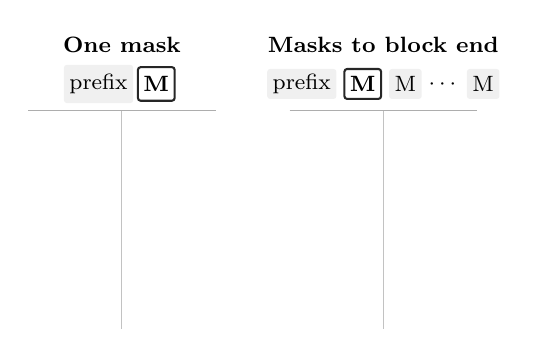
\begin{tikzpicture}[x=1cm,y=1cm,font=\small,
  token/.style={fill=black!6,rounded corners=1pt,minimum height=.38cm,inner xsep=2pt,font=\footnotesize},
  target/.style={token,draw=black!85,fill=white,line width=.75pt,font=\bfseries\footnotesize}]
\def\one{1.30}
\def\many{4.62}
% Each input heads one column. The guide passes through both measurements.
\foreach \x/\heading in {\one/One mask,\many/Masks to block end}{
  \node[font=\bfseries\footnotesize] at (\x,3.63) {\heading};
  \draw[black!32] ({\x-1.19},2.79)--({\x+1.19},2.79);
  \draw[black!24] (\x,2.79)--(\x,.02);}
\node[token,anchor=east] at ({\one+.15},3.13) {prefix};
\node[target,anchor=west] at ({\one+.19},3.13) {M};
\matrix[column sep=2.5pt,inner sep=0pt,ampersand replacement=\&] at (\many,3.13) {
  \node[token] {prefix}; \& \node[target] {M}; \& \node[token] {M}; \&
  \node[font=\footnotesize] {$\cdots$}; \& \node[token] {M}; \\
};
\def\noiseline#1#2#3#4#5#6{
  \coordinate (first) at (\one,{.15+5.65*(#5-1.30)});
  \coordinate (last) at (\many,{.15+5.65*(#6-1.30)});
  \draw[#1,thick,#2] (first)--(last);
  \foreach \point in {first,last}{\node[shape=#3,fill=#1,inner sep=0pt,minimum size=4pt] at (\point) {};}
  \node[left=4pt,text=#1,inner sep=0pt] at (first) {#5};
  \node[right=4pt,text=#1,inner sep=0pt] at (last) {#6};
  \node[anchor=west,xshift=4pt,#4,text=#1,inner sep=0pt,font=\footnotesize] at (first) {\modelname};}
\def\fixednoise#1#2{\def\modelname{Fixed noise range}\noiseline{black!75}{dashed}{rectangle}{yshift=-.47cm}{#1}{#2}}
\def\calibratednoise#1#2{\def\modelname{Calibrated range}\noiseline{blue!75!black}{solid}{circle}{yshift=.10cm}{#1}{#2}}
\drawnoise
\end{tikzpicture}
\end{minipage}\hfill
\begin{minipage}[t]{0.555\textwidth}
\raggedright\small
\textbf{B. The reference model favors repetition}\par
\smallskip
The two decoding policies use the same checkpoint, prompt and sampling seed.\par
\medskip
\noindent\textbf{Reuse the proposed token}\hfill{\footnotesize Full-text perplexity \textbf{\reusesampleppl}}\par
\smallskip
\noindent\textbf{Draw a fresh token}\hfill{\footnotesize Full-text perplexity \textbf{\freshsampleppl}}\par
\medskip
\noindent\textbf{Across all 32 prompts}\par
\smallskip
\begin{tabular*}{\linewidth}{@{\extracolsep{\fill}}lrr@{}}
\toprule
& Reuse proposal & Fresh draw \\
\midrule
Repeated four-grams & \reuserepeatrange & \textbf{\freshrepeatrange} \\
Reference perplexity & \textbf{\reusepplrange} & \freshpplrange \\
\bottomrule
\end{tabular*}
\end{minipage}
\caption{\textbf{Evaluation can reverse the choice of training method or decoder.} A averages next-token loss over 32 documents and two 20M checkpoints per noise policy. B holds the 20M checkpoint, prompt and sampling seed fixed. Both decoders sample without truncation and select up to four positions per pass. One keeps the proposals and the other redraws them \citep{zhang2026generatedtext}. Gemma 4 31B scores complete continuations. Ranges span two training seeds (32 prompts, two draws each). Bold marks the lower value.}
\label{fig:evaluation-choices}
\end{figure*}

\clearpage
\begin{table*}[!t]
\input{tables/final-model-rows}
\centering\small
\setlength{\tabcolsep}{3pt}
\renewcommand{\arraystretch}{1.12}
\begin{tabular}{@{}lrlrrrrrr@{}}
\toprule
 & \multicolumn{1}{c}{21 tasks} & \multicolumn{7}{c}{Sampled continuations at block length 32} \\
\cmidrule(lr){2-2}\cmidrule(l){3-9}
Training recipe & Acc. (\%) & Decoder (cap) & Tokens/fwd & Tokens/s & Ref. PPL & Ref. BPB & Repeat-4 (\%) & EOS \\
\midrule
\exhibitrows
\bottomrule
\end{tabular}
\caption{\textbf{Task accuracy and generation at 477M parameters.} Accuracy averages 21 separately scored tasks. Within each diffusion checkpoint, we time left-to-right decoding (top-$p=1$) and confidence-selected redrawing (top-$p=0.9$) on one A100-SXM4-80GB. Tokens/s averages per-request rates including cache work in BF16 autocast. Gemma 4 31B scores the continuations per token (PPL) and per byte (BPB). Repeat-4 averages the percentage of repeated four-grams per continuation. EOS counts stops before 256 tokens (32 prompts, two draws each).}
\label{tab:final-models}
\end{table*}

\clearpage
\begin{table*}[t]
\input{tables/study-design-rows}
\centering\small
\begin{tabular}{@{}p{.20\textwidth}p{.35\textwidth}p{.38\textwidth}@{}}
\toprule
Comparison & Training design & What the comparison measures \\
\midrule
\exhibitrows
\bottomrule
\end{tabular}
\caption{Experimental series and primary readouts. TPP is the number of allocated source tokens per counted parameter, including any AR pretraining. Within each series, candidates and controls share an evaluator.}
\label{tab:study-design}
\end{table*}

\clearpage
\begin{table*}[t]
\input{tables/model-size-rows}
\centering\small
\begin{tabular}{@{}rrrr@{}}
\toprule
Layers & Width & Total parameters (M) & Counted parameters $N_b$ (M) \\
\midrule
\exhibitrows
\bottomrule
\end{tabular}
\caption{Plain backbone sizes. A stage with budget $h$ TPP receives $hN_b$ allocated source tokens.}
\label{tab:model-sizes}
\end{table*}

\clearpage
\begin{figure*}[t]
\centering
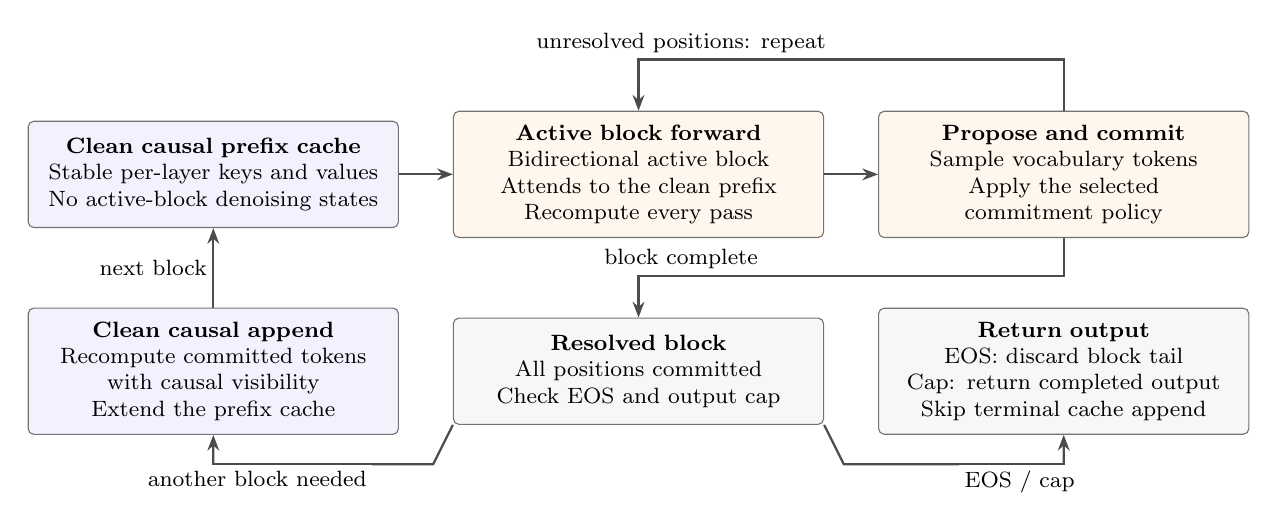
\begin{tikzpicture}[
  box/.style={draw=black!55, rounded corners=2pt, text width=4.35cm, minimum height=1.35cm, align=center, inner sep=5pt, font=\footnotesize},
  flow/.style={-{Stealth[length=2mm]}, thick, draw=black!70},
  lab/.style={font=\footnotesize, fill=white, inner sep=2pt}
]
\node[box,fill=blue!5] (cache) at (0,0) {\textbf{Clean causal prefix cache}\\Stable per-layer keys and values\\No active-block denoising states};
\node[box,fill=orange!7] (active) at (5.4,0) {\textbf{Active block forward}\\Bidirectional active block\\Attends to the clean prefix\\Recompute every pass};
\node[box,fill=orange!7] (sample) at (10.8,0) {\textbf{Propose and commit}\\Sample vocabulary tokens\\Apply the selected commitment policy};
\node[box,fill=blue!5] (append) at (0,-2.5) {\textbf{Clean causal append}\\Recompute committed tokens\\with causal visibility\\Extend the prefix cache};
\node[box,fill=black!3] (final) at (5.4,-2.5) {\textbf{Resolved block}\\All positions committed\\Check EOS and output cap};
\node[box,fill=black!3] (stop) at (10.8,-2.5) {\textbf{Return output}\\EOS: discard block tail\\Cap: return completed output\\Skip terminal cache append};
\draw[flow] (cache) -- (active);
\draw[flow] (active) -- (sample);
\draw[flow] (sample.north) -- ++(0,0.65) -| node[lab,pos=0.45,above]{unresolved positions: repeat} (active.north);
\draw[flow] (sample.south) -- ++(0,-0.48) -| node[lab,pos=0.45,above]{block complete} (final.north);
\draw[flow] (final.south west) -- ++(-0.25,-0.5) -| node[lab,pos=0.4,below]{another block needed} (append.south);
\draw[flow] (append) -- node[lab,left]{next block} (cache);
\draw[flow] (final.south east) -- ++(0.25,-0.5) -| node[lab,pos=0.4,below]{EOS / cap} (stop.south);
\end{tikzpicture}
\caption{\textbf{Flexible block generation with causal-prefix reuse.} Blue boxes contain clean reusable state; orange boxes contain temporary denoising state. The active block can change length between iterations of the outer loop. Only a clean causal append creates entries for future blocks; the final denoising pass cannot be cached directly. Prefix prefill occurs once before this loop.}
\label{fig:block-cache}
\end{figure*}

\clearpage
\begin{figure*}[p]
\centering
\input{figures/hp-grid-marks}
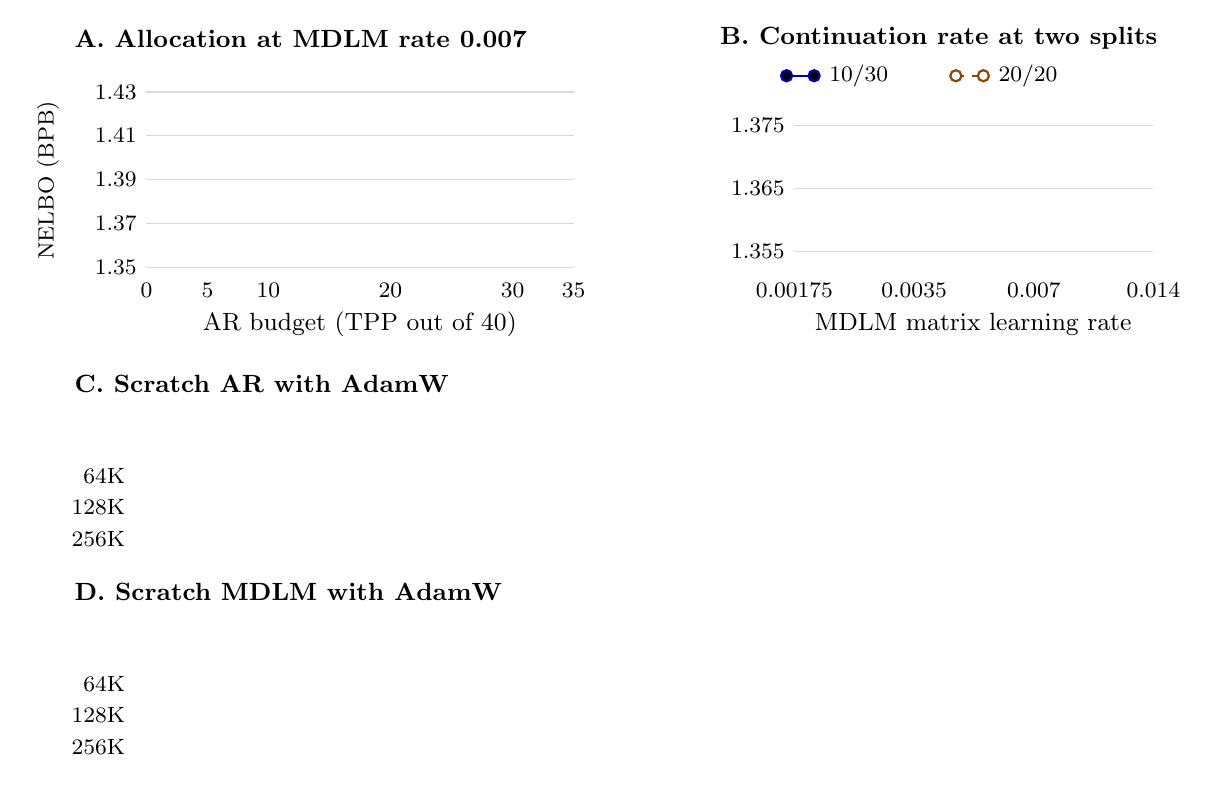
\begin{tikzpicture}[font=\small,
  allocation/.style={thick,draw=teal!70!black,mark=*},
  quarter/.style={thick,draw=blue!70!black,mark=*},
  half/.style={thick,dashed,draw=orange!55!black,mark=*,mark options={solid,fill=white,draw=orange!55!black}},
  heading/.style={anchor=west,font=\small\bfseries,inner sep=0pt},
  tick/.style={font=\footnotesize}]
\node[heading] at (0,3.85) {A. Allocation at MDLM rate 0.007};
\node[rotate=90,tick] at (-0.33,2.05) {NELBO (BPB)};
\node[heading] at (8.2,3.85) {B. Continuation rate at two splits};
\begin{scope}[shift={(0.92,0.95)},x=0.155cm,y=27.8cm]
  \pgftransformshift{\pgfpointxy{0}{-1.35}}
  \foreach \y in {1.35,1.37,1.39,1.41,1.43}{
    \draw[black!15] (0,\y)--(35,\y);
    \node[left,tick] at (0,\y) {\y};}
  \allocationcurve
  \foreach \x in {0,5,10,20,30,35}{\node[below,tick] at (\x,1.347) {\x};}
\end{scope}
\node at (3.63,0.22) {AR budget (TPP out of 40)};
\begin{scope}[shift={(9.15,0.95)},x=1.52cm,y=80cm]
  \pgftransformshift{\pgfpointxy{0}{-1.3525}}
  \foreach \y in {1.355,1.365,1.375}{
    \draw[black!15] (0,\y)--(3,\y);
    \node[left,tick] at (0,\y) {\y};}
  \quartercurve
  \halfcurve
  \foreach \x/\lr in {0/0.00175,1/0.0035,2/0.007,3/0.014}{
    \node[below,tick] at (\x,1.3515) {\lr};}
\end{scope}
\node at (11.42,0.22) {MDLM matrix learning rate};
\draw[quarter] plot coordinates {(9.05,3.38)(9.40,3.38)};
\node[right,tick] at (9.47,3.38) {10/30};
\draw[half] plot coordinates {(11.2,3.38)(11.55,3.38)};
\node[right,tick] at (11.62,3.38) {20/20};

\definecolor{scoreblue}{RGB}{108,179,192}
\def\budgettitle#1#2{\node[font=\footnotesize\bfseries] at ({3.24*#1+1},1.75) {#2 TPP};}
\def\ratelabel#1#2{\node[tick] at (#1,0.93) {#2};}
\def\scorecell#1#2#3#4{%
  \fill[scoreblue!#4] ({#1-.49},{#2-.48}) rectangle ({#1+.49},{#2+.48});
  \node[tick] at (#1,#2) {#3};}
\def\gridpanel#1#2#3{%
  \node[heading] at (0,{#1+1.17}) {#2};
  \begin{scope}[shift={(1.32,#1)},x=1.07cm,y=.40cm]
    \foreach \y/\batch in {0/64K,-1/128K,-2/256K}{
      \node[left,tick] at (-.51,\y) {\batch};}
    #3
  \end{scope}}
\gridpanel{-1.70}{C. Scratch AR with AdamW}{\argrid}
\gridpanel{-4.34}{D. Scratch MDLM with AdamW}{\mdlmgrid}
\end{tikzpicture}
\caption{\textbf{Training grids at 20M parameters.} A and B show document-start NELBO in bits per byte (BPB) for the Muon study. A varies the AR share at fixed total budget. B varies the MDLM rate for two AR/MDLM splits. C and D show the separate scratch AdamW grids. Rows give tokens per update (K means 1,024). Within each budget, columns give peak learning rate in units of $10^{-3}$. Cells show validation BPB, with darker shading for lower loss within each panel. C measures causal log loss and D measures masked reconstruction. Each panel uses one training seed. The companion tables give exact rates and scores for all tested cells.}
\label{fig:hp-grids}
\end{figure*}

\clearpage
\input{tables/d4-development-seeds}
\clearpage
\def\thepart{B}\refstepcounter{part}\label{app:replication-refresh}
\begin{table*}[t]
\input{tables/replication-coverage-rows}
\centering\small
\begin{tabular}{@{}p{.17\textwidth}p{.39\textwidth}p{.37\textwidth}@{}}
\toprule
Work & Intervention and comparison & What the 20M experiment shows \\
\midrule
\exhibitrows
\bottomrule
\end{tabular}
\caption{Scope of the small-model reconstructions. The first five rows cover the LLaDA family. Each row describes a component we could implement on our own data and backbone.}
\label{tab:replication-coverage}
\end{table*}

\clearpage
\input{tables/replication-refresh-seeds}
\clearpage
\input{tables/fastv2-compute}
\clearpage
\begin{figure*}[t]
\centering
\input{figures/scaling}
\caption{\textbf{The half-AR recipe has a lower full-sequence diffusion bound than scratch at six sizes.} Both recipes use AdamW and receive 40 tokens per counted parameter in total, including AR pretraining. The left panel includes the actual AR parents, trained for 20 tokens per counted parameter and scored with causal cross-entropy. The right panel compares only the two diffusion endpoints at each size. Each endpoint has one training seed and each diffusion score averages four corruption plans.}
\label{fig:scaling}
\end{figure*}

\clearpage
\input{tables/full-sequence-lr-transfer}
\clearpage
\begin{figure*}[t]
\centering
\resizebox{\textwidth}{!}{\input{figures/block-scaling}}
\caption{\textbf{AR pretraining for block diffusion at four model sizes.} Circles show block diffusion trained from scratch for 40 tokens per counted parameter. Squares show the same total budget split between AR pretraining (10) and block diffusion (30). Diamonds show the AR parent at the end of its 10-token budget. The left panel scores the next gold token given its prefix. The right panel scores reconstruction of partially masked blocks. Both use the same 32 documents and lower BPB is better. Diffusion points at 59M average three child-training seeds. All other points represent one checkpoint each. Figure~\ref{fig:block-scaling} reports the paired differences.}
\label{fig:block-absolute}
\end{figure*}

\clearpage
\begin{table*}[t]
\input{tables/block-rate-rows}
\centering\small
\begin{tabular}{@{}lrcccc@{}}\toprule
& Source tokens & \multicolumn{4}{c}{Peak matrix learning rate} \\
\cmidrule(l){3-6}
Training recipe & per update & 0.00175 & 0.0035 & 0.007 & 0.014 \\
\midrule
\exhibitrows
\bottomrule
\end{tabular}
\caption{All 59M discovery settings (seed 50). Each cell gives next-token BPB / reconstruction BPB on the same 32 development documents. Dashes mark untested cells. For conversion the lowest next-token loss occurs at the smallest tested rate and largest batch. For scratch the best rate falls inside the tested range.}
\label{tab:block-rate-search}
\end{table*}

\clearpage
\input{tables/block-holdout}
\clearpage
\input{tables/block-tasks}
\clearpage
\begin{table*}[t]
\input{tables/decoding-control-rows}
\centering\small
\setlength{\tabcolsep}{4pt}
\begin{tabular}{@{}lrr rr rr rr rr rr@{}}
\toprule
Size & Cap $K$ & Block & \multicolumn{2}{c}{Ref. PPL} & \multicolumn{2}{c}{Ref. BPB} & \multicolumn{2}{c}{Repeat-4 (\%)} & \multicolumn{2}{c}{EOS / 64} & \multicolumn{2}{c}{Tokens/fwd} \\
\cmidrule(lr){4-5}\cmidrule(lr){6-7}\cmidrule(lr){8-9}\cmidrule(lr){10-11}\cmidrule(l){12-13}
& & length & S & C & S & C & S & C & S & C & S & C \\
\midrule
\exhibitrows
\bottomrule
\end{tabular}
\caption{Generation at each tested block length. Each metric pairs scratch (S) with AR-initialized diffusion (C) on the same 32 prompts and two sampling seeds. The EOS columns count natural stops before 256 content tokens.}
\label{tab:decoding-controls}
\end{table*}

\clearpage
\begin{figure*}[t]
\centering
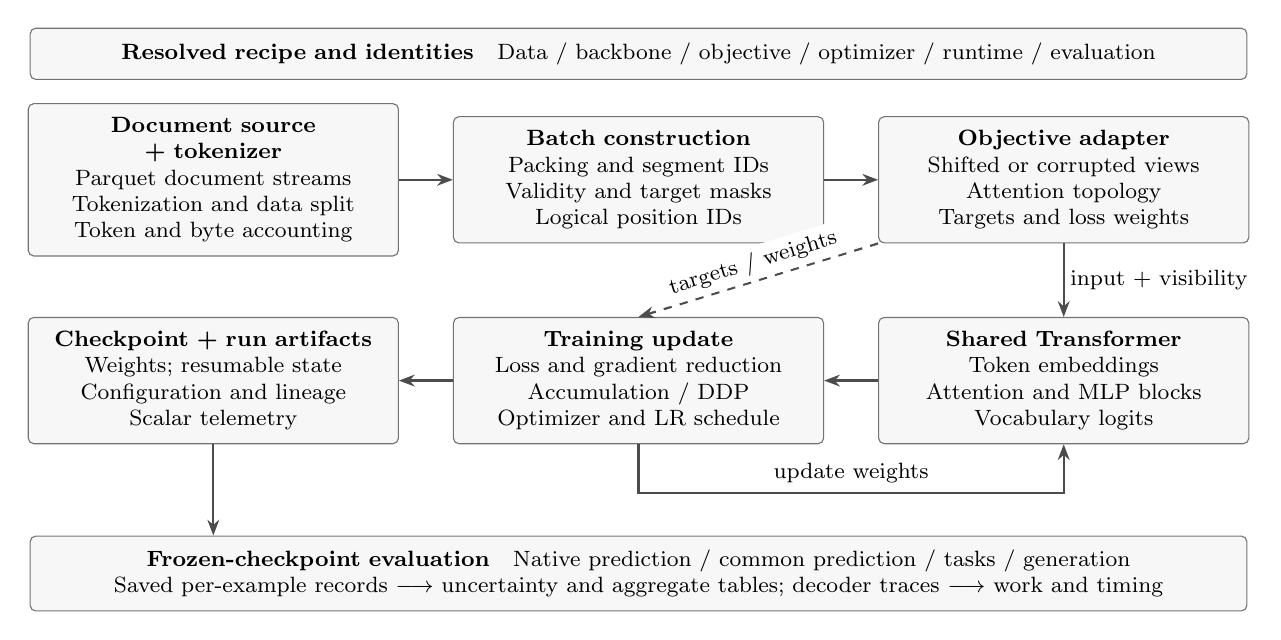
\begin{tikzpicture}[
  box/.style={draw=black!55, rounded corners=2pt, fill=black!3, text width=4.35cm, minimum height=1.45cm, align=center, inner sep=5pt, font=\footnotesize},
  flow/.style={-{Stealth[length=2mm]}, thick, draw=black!70},
  lab/.style={font=\footnotesize, fill=white, inner sep=2pt}
]
\node[box, text width=15.1cm, minimum height=0.65cm] (config) at (5.4,1.6) {\textbf{Resolved recipe and identities}\quad Data / backbone / objective / optimizer / runtime / evaluation};
\node[box] (source) at (0,0) {\textbf{Document source + tokenizer}\\Parquet document streams\\Tokenization and data split\\Token and byte accounting};
\node[box] (batch) at (5.4,0) {\textbf{Batch construction}\\Packing and segment IDs\\Validity and target masks\\Logical position IDs};
\node[box] (objective) at (10.8,0) {\textbf{Objective adapter}\\Shifted or corrupted views\\Attention topology\\Targets and loss weights};
\node[box] (artifacts) at (0,-2.55) {\textbf{Checkpoint + run artifacts}\\Weights; resumable state\\Configuration and lineage\\Scalar telemetry};
\node[box] (trainer) at (5.4,-2.55) {\textbf{Training update}\\Loss and gradient reduction\\Accumulation / DDP\\Optimizer and LR schedule};
\node[box] (model) at (10.8,-2.55) {\textbf{Shared Transformer}\\Token embeddings\\Attention and MLP blocks\\Vocabulary logits};
\node[box, text width=15.1cm, minimum height=0.9cm] (eval) at (5.4,-5.0) {\textbf{Frozen-checkpoint evaluation}\quad Native prediction / common prediction / tasks / generation\\Saved per-example records $\longrightarrow$ uncertainty and aggregate tables; decoder traces $\longrightarrow$ work and timing};
\draw[flow] (source) -- (batch);
\draw[flow] (batch) -- (objective);
\draw[flow] (objective) -- node[lab,right]{input + visibility} (model);
\draw[flow,dashed] (objective.south west) -- node[lab,above,sloped]{targets / weights} (trainer.north);
\draw[flow] (model.west) -- (trainer.east);
\draw[flow] (trainer.south) -- ++(0,-0.62) -| (model.south);
\node[lab] at (8.1,-3.72) {update weights};
\draw[flow] (trainer) -- (artifacts);
\draw[flow] (artifacts.south) -- (artifacts.south |- eval.north);
\end{tikzpicture}
\caption{\textbf{Platform interfaces.} The recipe configures the components; arrows show the main data and training flow. Objective adapters own visibility and supervision, while the shared backbone owns network computation. Evaluation reads a fixed checkpoint independently of the training loop. The diagram is an interface map, not a claim that every combination is supported.}
\label{fig:platform-system}
\end{figure*}

\clearpage
\input{tables/components}
\clearpage
\input{tables/estimator-screen}
\clearpage
\input{tables/repair-screen}
\clearpage
\input{tables/component-seeds}
\clearpage
\input{tables/generation-d4}
\clearpage
\input{tables/ar-grid}
\clearpage
\input{tables/mdlm-grid}
\clearpage
\input{tables/context}
\clearpage
\input{tables/d12-muon}
\clearpage
\input{tables/d20-recipes}
\clearpage
\input{tables/d20-prediction}
\clearpage
\input{tables/d20-generation}
\clearpage
\input{tables/d20-tasks}
\clearpage
\input{tables/d4-development}
\clearpage
\input{tables/d4-hp-allocation}
\clearpage
\input{tables/d4-hp-schedule}
\clearpage
\input{tables/d4-hp-batch}
\clearpage
\input{tables/replication-refresh}
\clearpage
\input{tables/replication-refresh-generation}
\clearpage
\input{tables/fastv2-compute-generation}
\clearpage
\input{tables/block-prediction}
\clearpage
\input{tables/block-seeds}
\clearpage
\input{tables/block-d8-grid}
\clearpage
\input{tables/block-intervals}
\clearpage
\input{tables/block-tasks-main}
\clearpage
\input{tables/block-task-controls}
\clearpage
\input{tables/block-generation}
\clearpage
\input{tables/block-generation-lengths}
\clearpage
\input{tables/block-d8-generation}
\clearpage
\input{tables/block-runtime}
\clearpage
\input{tables/scaling}
\clearpage
\begin{thebibliography}{2}
\bibitem[Jain(2026)]{jain2026adaptive} Gagan Jain. Adaptive Block Diffusion: Resolving Training-Inference Mismatch in Diffusion Language Models. arXiv:2606.29275.
\bibitem[Zhang et al.(2026)]{zhang2026generatedtext} Zeyang Zhang et al. Differences in Text Generated by Diffusion and Autoregressive Language Models. arXiv:2605.12522.
\end{thebibliography}
\end{document}
